%!TEX program = xelatex
%!TEX options = --shell-escape

\documentclass{article}
\usepackage{fontenc}
\usepackage{minted}
\usepackage{upquote}
\setminted{fontsize=\small}
 \setminted[json]{fontsize=\footnotesize}
 \setminted[shell]{fontsize=\small}
\usepackage{graphicx}
\graphicspath{{image/}{figure/}{fig/}{img/}}
\usepackage[a4paper,margin=2.5cm]{geometry}
\usepackage[dvipsnames]{xcolor}
\usepackage{hyperref}
\hypersetup{
  colorlinks,
  citecolor=Violet,
  linkcolor=Red,
  urlcolor=NavyBlue}
\usepackage{xeCJK}
\usepackage{fontspec,xunicode,xltxtra}
 \setmainfont{LibertinusSerif-Regular}
 \setsansfont{LibertinusSans-Regular}
%  \setmonofont{Ubuntu Mono}
% \usepackage{FiraMono}
\setCJKmainfont[ItalicFont={FZKTJW.ttf}, BoldFont={FZHTJW.ttf}]{FZSSJW.ttf}
\setCJKsansfont[BoldFont={FZHTJW.ttf}]{FZKTJW.ttf}
\setCJKmonofont{FZKTJW.ttf}

\usepackage{indentfirst}
\setlength{\parindent}{2em}

\usemintedstyle{elegant}
\linespread{1.3}
\usepackage{etoolbox,xpatch}

\makeatletter
\AtBeginEnvironment{minted}{\dontdofcolorbox}
\def\dontdofcolorbox{\renewcommand\fcolorbox[4][]{##4}}
\xpatchcmd{\inputminted}{\minted@fvset}{\minted@fvset\dontdofcolorbox}{}{}
\makeatother

% caption settings 
\RequirePackage[font=small,labelfont={bf}]{caption} 
\captionsetup[table]{skip=3pt}
\captionsetup[figure]{skip=3pt}

% list/itemize/enumerate setting
\RequirePackage[shortlabels]{enumitem}
\setlist{nolistsep}

\renewcommand{\figurename}{\bfseries 图}
\renewcommand{\tablename}{\bfseries 表}

\title{\bfseries \LaTeX{} 编译环境配置:Visual Studio Code 配置简介}
\author{\href{https://ddswhu.me/}{Dongsheng Deng}}
\date{\today}

\begin{document}
\maketitle

本文介绍如何配置 Visual Studio Code 作为 \LaTeX{} 的编辑器。Github 地址:\href{https://github.com/EthanDeng/vscode-latex}{vscode-latex},欢迎提交 issues 和 pull requests。

\section{为什么用 Visual Studio Code}
Visual Studio Code(以下简称 VS Code) 是微软推出的一个编辑器,它的优点你可以自行百度,这里不赘述。对我来说,它最有吸引力的当属在 Windows 系统,它对于中英文字体的渲染。如果你原来用过其他编辑器,你就知道在普通屏幕上,中英文的显示效果简直是灾难。我原来因为编辑器的中文显示(当然还有 Terminal 的吸引力)一度想买 Mac,当然最后因为对性能和颜值的追求并不匹配我的财力,加上 Windows 上有些软件不能舍弃,最后作罢。

\textbf{注}:高分屏加上合适的字体,Sublime Text 的显示效果也非常好。

\begin{figure}[htbp]
  \centering
  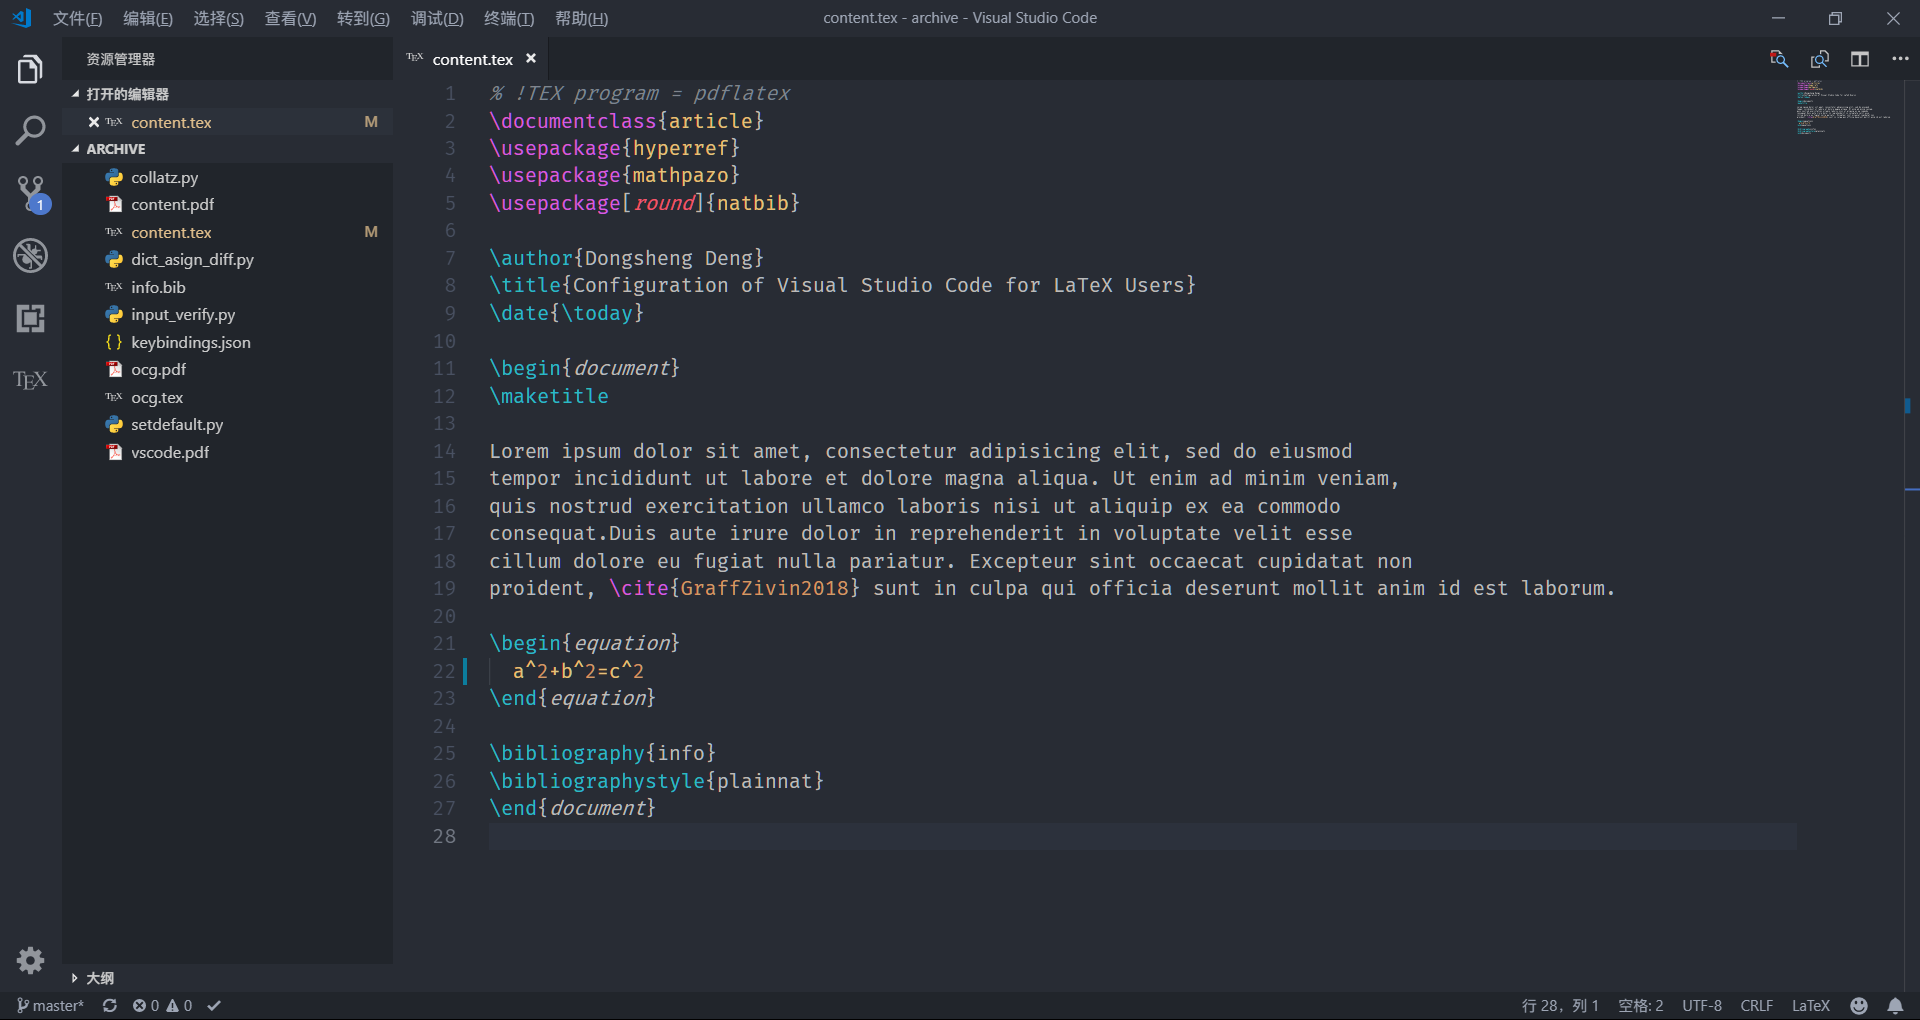
\includegraphics[width=0.9\textwidth]{vscode.png}
  \caption{Visual Studio Code 的界面图}
  \label{fig:vscode}
\end{figure}



\section{准备工作}
首先,为了搭建 \LaTeX{} 工作环境,你需要安装:

\begin{itemize}
  \item \TeX{} Live 或者 MiKTeX (本文以 \TeX{} Live 2018 为例)
  \item Visual Studio Code
  \item \LaTeX{} Workshop (VS Code 插件)
  \item SumatraPDF 阅读器(可选,用于预览 PDF)
\end{itemize}

在上述软件/插件安装之后,你需要把 \TeX{} Live 的 bin 目录(\mintinline[breaklines]{shell}{D:/Program Files/texlive/2018/bin/win32}) 以及 SumatraPDF 的路径(\mintinline[breaklines]{shell}{C:/Program Files (x86)/SumatraPDF})添加到系统环境变量(\mintinline{shell}{Path})中。


\subsection{安装插件}
VS Code 中插件安装方法如下:在左侧点击扩展按钮(Key:\mintinline{shell}{Ctrl+Shift+X}),然后搜索插件名字 \mintinline{shell}{LaTeX Workshop},选择安装即可。

\subsection{添加环境变量}
Win10 中将路径添加到环境变量中的步骤如下:右键我的电脑,然后选择 \mintinline{shell}{属性},在左侧选择 \mintinline{shell}{高级系统设置},然后选择下方的 \mintinline{shell}{环境变量},选择变量 \mintinline{shell}{Path} 编辑,将需要添加的路径添加进去即可。

\section{配置编译方式与编译组合}
VS Code 在 2018 年经历了一次大改之后,配置比原来简单了。它们把过去的 \mintinline{shell}{tool.chain} 改为了 \mintinline{shell}{recipe},其实本质上是一样的。

\subsection{编译方式(tool)}
VS Code 默认添加了 3 个编译工具(tools):分别是 \mintinline{shell}{latexmk},\mintinline{shell}{pdflatex} 和 \mintinline{shell}{bibtex}(所有的工具只编译一次)。编译 \mintinline{shell}{tex} 文档方法,使用右键,选择 \mintinline{shell}{Build LaTeX Project}(快捷键:\mintinline{shell}{Ctrl+Alt+B}),默认使用 \mintinline{shell}{latexmk},查看 PDF 文件使用快捷键:\mintinline{shell}{Ctrl+Alt+V}。

为了添加其他的编译方式(比如 \mintinline{shell}{xelatex}),我们需要修改 \LaTeX{} Workshop 的配置。打开 LaTeX Workshop 配置的方法如下:在 VS Code 界面左下角,点击齿轮按钮 
\includegraphics[width=0.018\textwidth]{setting.png},选择\mintinline{shell}{设置},然后在设置搜索框内输入 \mintinline{shell}{latex},在搜索结果中,点击 \underline{\mintinline{shell}{在 settings.json 中编辑}},示例如图~\ref{fig:settings}:

\begin{figure}[!htbp]
  \centering
  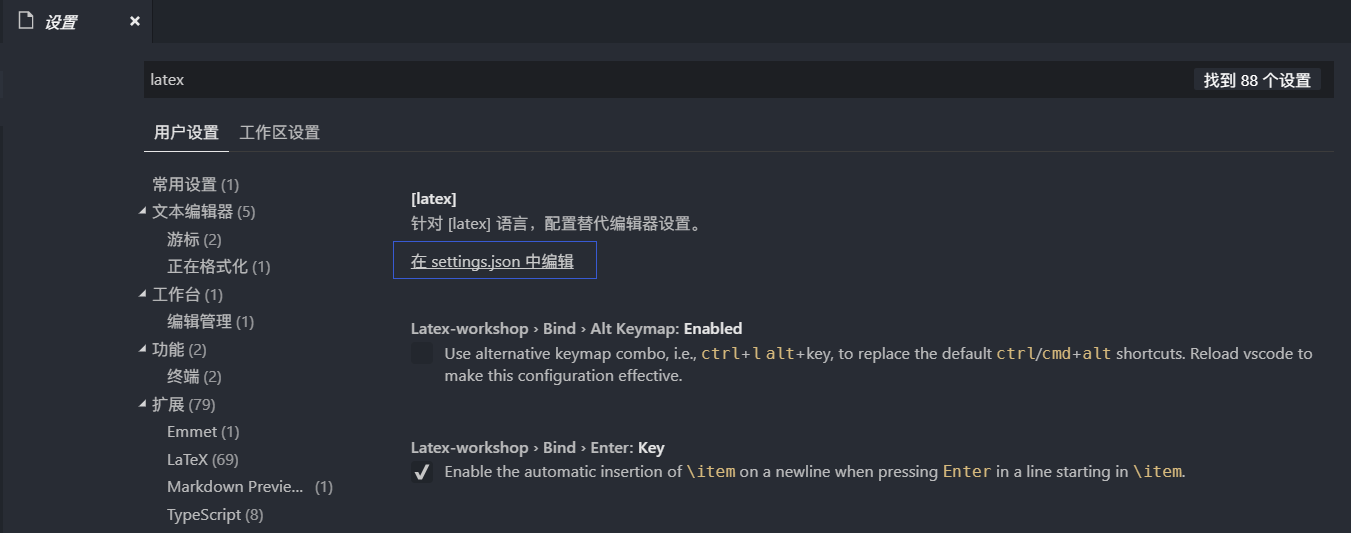
\includegraphics[width=0.7\textwidth]{settings.png}
  \caption{打开设置文件\label{fig:settings}}
\end{figure}


打开配置文件之后,在右侧 \mintinline{shell}{用户设置} 粘贴\footnote{最好从 \mintinline{shell}{main.tex} 里面拷贝,注意,引号全部为英文引号。}下面 JSON 片段\footnote{粘贴在 \mintinline{shell}{]} 之前,务必保证 JSON 格式的完整性。}:

\begin{minted}[frame=single]{json}
"latex-workshop.latex.tools": [
  {
    "name": "xelatex",
    "command": "xelatex",
    "args": [
      "-synctex=1",
      "-interaction=nonstopmode",
      "-file-line-error",
      "%DOC%"
    ]
  },
  {
    "name": "xelatex-with-shell-escape",
    "command": "xelatex",
    "args": [
      "--shell-escape",
      "-synctex=1",
      "-interaction=nonstopmode",
      "-file-line-error",
      "%DOC%"
    ]
  },
  {
    "name": "pdflatex",
    "command": "pdflatex",
    "args": [
      "-synctex=1",
      "-interaction=nonstopmode",
      "-file-line-error",
      "%DOC%"
    ]
  },
  {
    "name": "pdflatex-with-shell-escape",
    "command": "pdflatex",
    "args": [
      "--shell-escape",
      "-synctex=1",
      "-interaction=nonstopmode",
      "-file-line-error",
      "%DOC%"
    ]
  },
  {
    "name": "latexmk",
    "command": "latexmk",
    "args": [
      "-synctex=1",
      "-interaction=nonstopmode",
      "-file-line-error",
      "-pdf",
      "%DOC%"
    ]
  },
  {
    "name": "bibtex",
    "command": "bibtex",
    "args": [
      "%DOCFILE%"
    ]
  },
  {
    "name":"makeindex",
    "command":"makeindex",
    "args":[
        "%DOCFILE%"
    ]
  },
],
\end{minted}

\textbf{注意:}虽然左侧插件默认添加了编译方式(\mintinline{shell}{pdflatex} 与 \mintinline{shell}{bibtex}),也必须将其编译方式的设置(比如 \mintinline{shell}{pdflatex} 等)添加到右侧用户设置中。另外上面我们分别为 \mintinline{shell}{pdflatex} 和 \mintinline{shell}{xelatex} 添加了 \mintinline{shell}{--shell-escape} 参数,一个典型的应用场景就是编译包含 \mintinline{tex}{minted} 宏包的文件时。

\subsection{编译组合(recipe)}
如果我们要对一个文档/项目完整的编译(比如 \mintinline[breaklines]{shell}{pdflatex -> bibtex -> pdflatex -> pdflatex})我们需要用到编译组合(\mintinline{shell}{recipes})。LaTeX Workshop 默认添加了两个 \mintinline{shell}{recipes},分别是 \mintinline{shell}{latexmk} 和 \mintinline[breaklines]{shell}{pdflatex -> bibtex -> pdflatex*2},可以通过点击左侧新增的 \TeX{} 按钮 
\includegraphics[width=0.028\textwidth]{tex.png},然后点击 \mintinline{shell}{Build LaTeX project},选择适合的编译组合。


\begin{figure}[htbp]
  \centering
  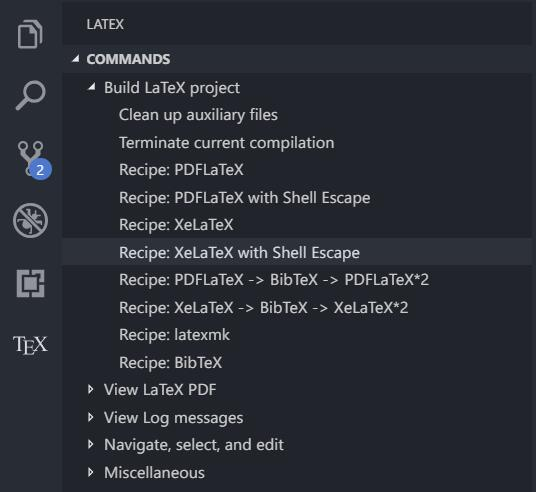
\includegraphics[width=0.5\textwidth]{compile.jpg}
  \caption{编译组合的选择}
  \label{fig:Compilation combination selection}
\end{figure}


我们之前添加了 \mintinline{shell}{xelatex} 编译方式,我们这里配置下 \mintinline{shell}{xelatex} 的完整编译链 \mintinline[breaklines]{shell}{xelatex -> bibtex -> xelatex*2},另外补充单次编译的 \mintinline{shell}{recipes}。方法和之前类似,打开用户配置文件,将如下 JSON 添加到用户配置中即可。添加新的编译组合之后需要重启 VS Code 才能在 \TeX{} 按钮下看到。


\begin{minted}[frame=single]{json}
"latex-workshop.latex.recipes": [
  {
    "name": "PDFLaTeX",
    "tools": [
      "pdflatex"
    ]
  },
  {
    "name": "PDFLaTeX with Shell Escape",
    "tools": [
      "pdflatex-with-shell-escape"
    ]
  },
  {
    "name": "XeLaTeX",
    "tools": [
      "xelatex"
    ]
  },
  {
    "name": "XeLaTeX with Shell Escape",
    "tools": [
      "xelatex-with-shell-escape"
    ]
  },
  {
    "name": "PDFLaTeX -> BibTeX -> PDFLaTeX*2",
    "tools": [
      "pdflatex",
      "bibtex",
      "pdflatex",
      "pdflatex"
    ]
  },
  {
    "name": "XeLaTeX -> BibTeX -> XeLaTeX*2",
    "tools": [
      "xelatex",
      "bibtex",
      "xelatex",
      "xelatex"
    ]
  },
  {
    "name": "latexmk",
    "tools": [
      "latexmk"
    ]
  },
  {
    "name": "BibTeX",
    "tools": [
      "bibtex"
    ]
  },
  {
    "name":"MakeIndex",
    "tools":[
        "makeindex"
    ]
  },
],
\end{minted}

\mintinline{shell}{settings} 目录下提供了一个比较完整的配置文件 \href{https://github.com/EthanDeng/vscode-latex/blob/master/settings/settings.json}{settings.json},包括了 \mintinline{tex}{latexmk}\footnote{参考了啸行的《编辑器 texstudio 和 vscode 使用总结》} 与 \mintinline{shell}{pdflatex/xelatex} 以及 \mintinline{shell}{--shell-escape} 的搭配使用。需要的可以下载替换掉用户配置 \mintinline{shell}{tools} 和 \mintinline{shell}{recipe} 部分。另外 \mintinline{shell}{example} 目录下提供一个测试完整编译方式的代码 \href{https://github.com/EthanDeng/vscode-latex/blob/master/example/content.tex}{tex}, \href{https://github.com/EthanDeng/vscode-latex/blob/master/example/info.bib}{bib}, \href{https://github.com/EthanDeng/vscode-latex/blob/master/example/content.pdf}{pdf},你可以用来测试能否编译。效果图如图~\ref{fig:example}:

\begin{figure}[htbp]
  \centering
  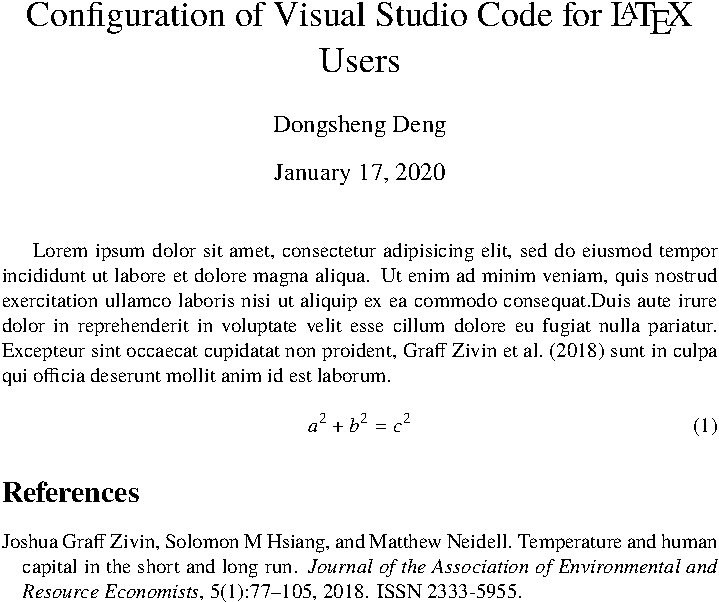
\includegraphics{example.pdf}
  \caption{编译效果图}
  \label{fig:example}
\end{figure}


\subsection{指定编译方式}
在 Sublime Text 或者 \TeX{} Studio 中,可以在文件的首行指定编译方式(\mintinline{shell}{% !TEX program})以及主文档(\mintinline{shell}{% !TEX root}),\LaTeX{} Workshop 也把这个功能添加到了其中,使用方法完全一样。\mintinline{shell}{% !TEX program} 和 \mintinline{shell}{% !TEX root} 被称为 Magic Command(魔法注释)。示例如下:


\begin{minted}[frame=single]{latex}
% !TEX program = xelatex
\documentclass{article}

\author{Dongsheng Deng}
\title{Configuration of Visual Studio Code for \LaTeX{} Users}

\begin{document}

\maketitle
Example text.

\end{document}
\end{minted}

将上述代码保存为 \mintinline{shell}{test.tex},然后使用快捷键 \mintinline{shell}{Ctrl+Alt+B},系统会自动选择 \mintinline{shell}{xelatex} 作为编译方式。如果没有其他问题,就能正常编译。




\section{其他配置}
\subsection{配置快捷键}
\LaTeX{} Workshop 的快捷键并不友好,我们可以自定义快捷键,方法如下:点击 VS Code 左下角的齿轮(设置),选择 \mintinline{shell}{键盘快捷方式}。


\begin{itemize}
  \item 搜索 \mintinline{shell}{latex build project},将默认的快捷方式改为 \mintinline{shell}{Ctrl+B}
  \item 搜索 \mintinline{shell}{latex build with recipe},将其改为 \mintinline{shell}{Ctrl+R}
  \item 搜索 \mintinline{shell}{latex view pdf file},将其改为 \mintinline{shell}{Ctrl+L}
  \item 你还可以补充其他快捷键。
\end{itemize}

配置好快捷键之后,之后当你指定了编译方式时可以直接使用快捷键 \mintinline{shell}{Ctrl+B} 编译一次文档。当你需要完整编译整个文档(文献,目录等),使用快捷键 \mintinline{shell}{Ctrl+R},选择完整的编译方案即可。是不是方便多了?

\textbf{补充}:为了方便快捷键的绑定,这里直接提供设置文件(\mintinline{shell}{keybindings.json})的 \href{https://github.com/EthanDeng/vscode-latex/blob/master/settings/keybindings.json}{下载},下载之后只需要将其替换用户的快捷键设置即可(默认位置为:\mintinline[breaklines]{shell}{C:/Users/<Your User Name>/AppData/Roaming/Code/User})。


\subsection{配置阅读器以及自动编译}
还有其他几个设置需要提一下,由于笔记本的屏幕很小,我并不习惯使用 VS Code 自带的 PDF 阅读器作为预览的阅读器,可以设置 \mintinline{shell}{SumatraPDF} 作为 PDF 阅读器\footnote{还可以设置 \mintinline{shell}{SumatraPDF} 与 VS Code 之间的正反跳转,详见\href{https://wenda.latexstudio.net/article-5055.html}{《\mintinline{shell}{SumatraPDF} 阅读器该怎么设置——以 TeXStudio 和 VS Code 为例》}}。

\begin{minted}[frame=single]{json}
"latex-workshop.view.pdf.viewer": "external",
\end{minted}

\subsection{Mac 系统 PDF 阅读器配置}
如何让 VS Code 在 Mac 上与诸如 Skim 的外部 PDF 浏览器配合工作——特别是 \LaTeX{} 的正反跳转,请参考小 L 的 \href{https://liam0205.me/2018/04/24/Working-with-VSCode-on-macOS-configuration-LaTeX-workshop-and-Skim/}{配置说明}。

\section*{参考资料}
\begin{itemize}
    \item 本文最早的版本 \href{http://www.latexstudio.net/archives/11087.html}{LaTeX 技巧 916:Visual Studio Code 搭建 LaTeX 编写环境(已被删)}.
    \item 更新版本为 \href{http://www.latexstudio.net/archives/12260.html}{LaTeX技巧932:如何配置Visual Studio Code作为LaTeX编辑器[新版更新]}
    \item \href{https://github.com/James-Yu/LaTeX-Workshop}{Github: LaTeX-Workshop}
    \item \href{https://stackoverflow.com/questions/39775406/how-to-turn-off-matching-highlighting}{How to turn off matching highlighting}
\end{itemize}


\end{document}
